%=============================--A--=============================%
\subsection{Módulo 1 $\pmb \mapsto$ Desmodulaç\~ao}
\label{subsec:mod1}

%\iffalse
\begin{figure}[H]
    \centering
    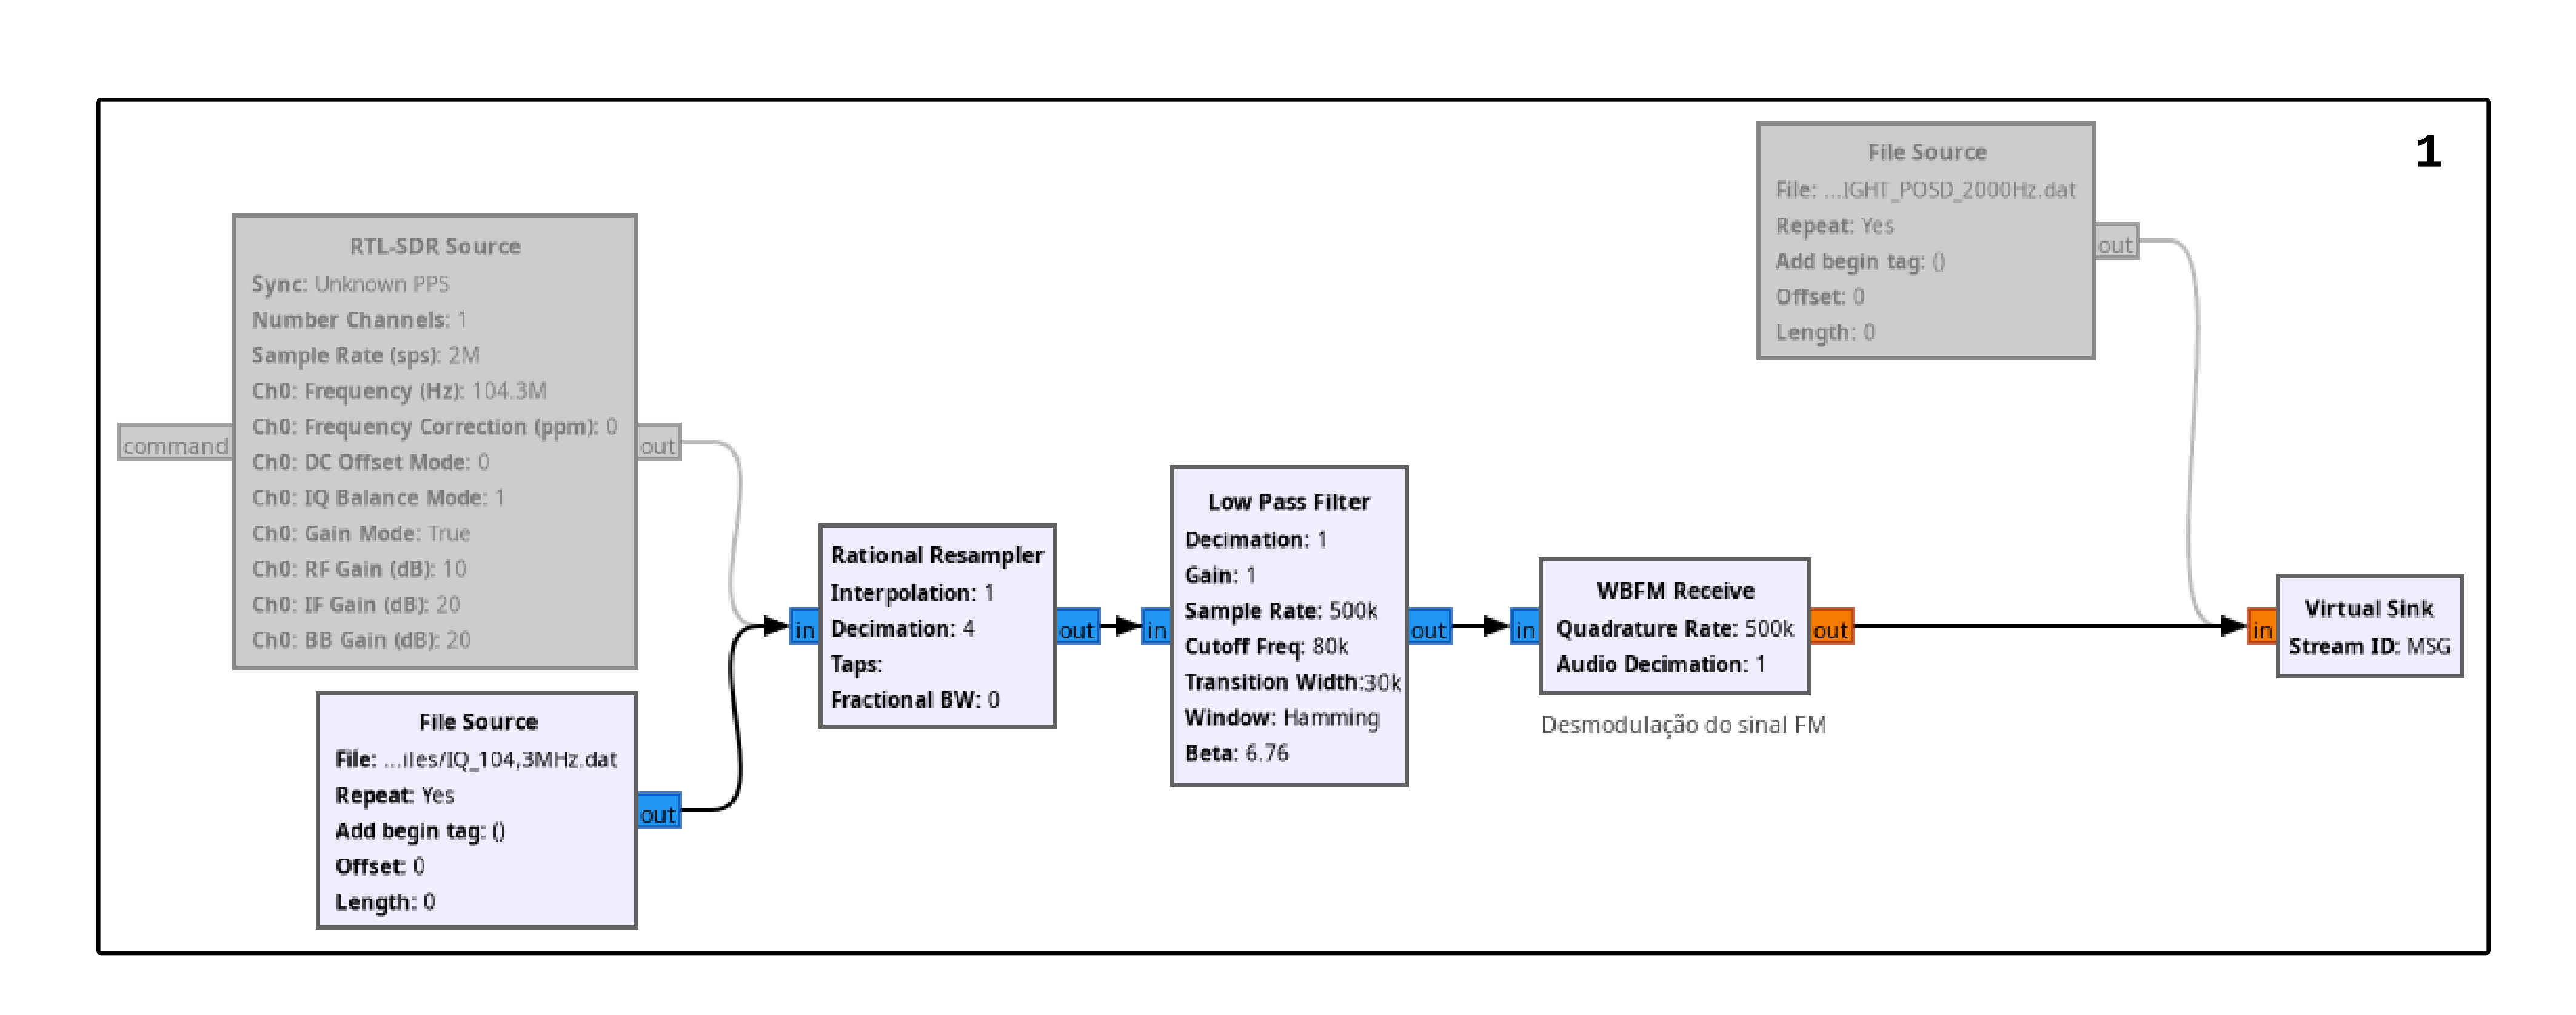
\includegraphics[width = 1\linewidth]{img/mods/modulo1.png}
    \caption{Processo de obtenção do sinal mensagem multiplexado $m(t)$.}
    \label{fig:modulo1}
\end{figure}
%\fi

Os sinais recebidos pela antena ou extraído dos ficheiros de testes (associado ao bloco "RTL-SDR Source" e "File Source" respetivamente), são sinais FM, logo no formato:

\begin{equation*}
    x_{FM}(t)=A_c \cos{(2\pi f_c t + 2 \pi k_f  \int_{-\infty}^{t} m(\lambda) \,d\lambda)}
\end{equation*}
 
Tal como já mencionado, na introdução, para desmodular um sinal FM utiliza-se um desmodulador em quadratura, que se encontra no bloco "WBFM Receive". Este também contém um filtro de de-ênfase (para compensar a pré-ênfase do processo de modulação) e um passa-baixo, que como já referido, melhoram significativamente a qualidade do sinal.

Dado que se optou por utilizar uma frequência de amostragem de $2$ MHz, ritmo aceitável para a interface USB que vai receber as amostras do sinal, antes do sinal ser desmodulado realiza-se uma redução da frequência de amostragem por um fator de 1/4, processo este realizado no bloco de "Rational Resampler". A posterior descodificação é feita com este ritmo de amostragem de $500$ kHz.

É importante realçar que este processo de desmodulação FM é igual ao apresentado no guia laboratorial (pág. 29), uma vez que independentemente da mensagem transmitida estar num formato mono ou stereo, o processo de desmodulação FM para a obtenção da mensagem $m(t)$ é o mesmo.

No final deste modulo é colocada a mensagem multiplexada $m(t)$ numa variável de nome MSG, com auxilio do bloco "Virtual Sink".

Faz-se o reparo que os sinais de teste fornecidos LEFT e RIGHT, já se apresentam desmodulados, pelo que apenas necessitam de ser desmultiplexados para a efetuação da calibração do delay, e assim, são diretamente direcionados para o "Virtual Sink".